\section{\filetotitle}\label{sec:variational_principles}
The numerical schemes described in Sec~\ref{sec:numerical_schemes_for_time_dependent_schrodinger_equation} are theoretically exact, but in practice, they require the representation of the full wavefunction. This is computationally infeasible for large quantum systems due to the exponential growth of grid points required to sample the wavefunction. The variational principles discussed in this section approximate the time evolution by projecting the dynamics onto a lower-dimensional smooth submanifold $\mathcal{M}\subset\mathcal{H}$. We define this manifold as the set of all trial wavefunctions parametrized by a complex vector $\symbf{\alpha}(t) \in \mathbb{C}^N$ as
\begin{equation}
\mathcal{M}=\lbrace\ket{\Psi(\symbf{\alpha})}:\symbf{\alpha}\in\mathbb{C}^N \}.
\end{equation}
This approach allows us to evolve the system's state using a manageable number of parameters $\symbf{\alpha}=(\alpha_1(t),\ldots,\alpha_N(t))$. In the following subsections, we will explore three key variational principles: the Dirac--Frenkel principle, McLachlan's variational principle, and the time-dependent variational principle.
\subsection{Dirac--Frenkel Principle}\label{sec:dirac_frenkel_principle}
The first variational principle we consider is the \acrfull{dfvp}. The exact time evolution is governed by the \acrshort{tdse}, $\partial_t\ket{\Psi}=-iH\ket{\Psi}$. However, the vector $-iH\ket{\Psi}$ generally leads out of the manifold $\mathcal{M}$. We therefore seek a time-derivative vector that lies strictly within the tangent space $T_{\Psi}\mathcal{M}$.

Formalizing this, the tangent space at a point $\ket{\Psi(\symbf{\alpha})}$ is spanned by the partial derivatives of the wavefunction with respect to the parameters
\begin{equation}
T_{\Psi}\mathcal{M}=\text{span}\left\lbrace\frac{\partial}{\partial\alpha_k}\ket{\Psi(\symbf{\alpha})}\right\rbrace_{k=1}^N.
\end{equation}
Consequently, the approximate time evolution of the state is given by the chain rule as
\begin{equation}\label{eq:tangent_evolution}
\partial_t\ket{\Psi\left(\symbf{\alpha}\right)}=\sum_{k=1}^N\dot{\alpha}_k\frac{\partial}{\partial\alpha_k}\ket{\Psi(\symbf{\alpha})}\in T_{\Psi}\mathcal{M}.
\end{equation}
The Dirac--Frenkel principle postulates that the optimal parameters $\dot{\symbf{\alpha}}$ are found by minimizing the distance between the exact dynamics and the tangent space evolution. We define the residual vector (the error) as
\begin{equation}
\ket{\epsilon}=\partial_t\ket{\Psi\left(\symbf{\alpha}\right)}+iH\ket{\Psi\left(\symbf{\alpha}\right)}.
\end{equation}
Minimizing the norm $\lvert\ket{\epsilon}\rvert^2$ with respect to the parameter variations $\dot{\symbf{\alpha}}$ implies that the residual vector must be orthogonal to the tangent space. The geometric interpretation of this projection is visualized in Fig~\ref{fig:dirac_frenkel_principle}.
\begin{figure}[H]
\centering
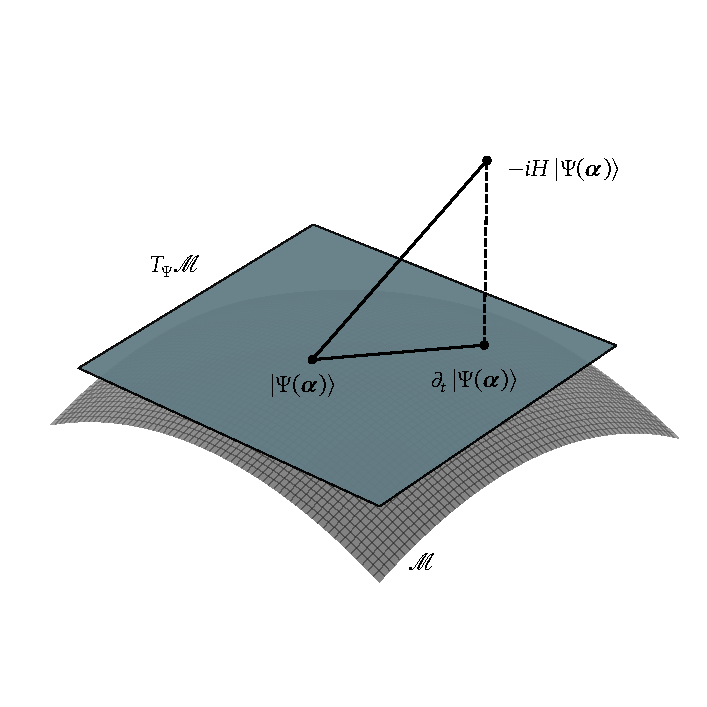
\includegraphics[clip,trim={0.7cm 2.1cm 0.5cm 2.0cm},width=.9\linewidth]{chapters/02-Time_Evolution_in_Quantum_Mechanics/sections/images/dfvp_schema}
\caption{The Dirac--Frenkel variational principle projects the exact time-derivative vector $-iH\ket{\Psi\left(\symbf{\alpha}\right)}$ onto the tangent space $T_{\Psi}\mathcal{M}$ to find the optimal approximate time evolution $\partial_t\ket{\Psi\left(\symbf{\alpha}\right)}$. The residual vector $\ket{\epsilon}$ (dashed line) is orthogonal to the tangent space $T_{\Psi}\mathcal{M}$.}
\label{fig:dirac_frenkel_principle}
\end{figure}
As illustrated, the exact time-derivative vector $-iH\ket{\Psi\left(\symbf{\alpha}\right)}$ is projected orthogonally onto $T_{\Psi}\mathcal{M}$ to find the optimal $\partial_t\ket{\Psi\left(\symbf{\alpha}\right)}$. Mathematically, the condition that the residual $\ket{\epsilon}$ is orthogonal to the tangent space requires that
\begin{equation}\label{eq:dfvp_orthogonality_condition}
\Braket{\delta\Psi|\partial_t+iH|\Psi\left(\symbf{\alpha}\right)}=0\quad\forall\ket{\delta\Psi}\in T_{\Psi}\mathcal{M},
\end{equation}
where $\ket{\delta\Psi}$ represents arbitrary variations within the tangent space. This equation constitutes the formal definition of the \acrshort{dfvp} and yields the equations of motion for the parameters $\symbf{\alpha}$.
\subsection{McLachlan's Variational Principle}\label{sec:mclachlan_variational_principle}
\subsection{Time-Dependent Variational Principle}\label{sec:time_dependent_variational_principle}
